\documentclass{beamer}
\usetheme{Boadilla}

\usepackage{graphicx}
\usepackage{subcaption}
\usepackage{csvsimple}

% Set relative path to all figures
\newcommand*{\floatRelativePath}{../out/gwas417/pval_5e-08/r2_0.1/kb_1000/window_1000000/75_50}%
% Footnote without marker: https://tex.stackexchange.com/questions/30720/footnote-without-a-marker
\newcommand\blfootnote[1]{%
    \begingroup
    \renewcommand\thefootnote{}\footnote{#1}%
    \addtocounter{footnote}{-1}%
    \endgroup
}
% Change size of footnotes
\renewcommand{\footnotesize}{\fontsize{5pt}{5pt}\selectfont}
% reset footnote counter for each frame in beamer class
\AtBeginEnvironment{frame}{\setcounter{footnote}{0}}

\title{Discovery and analysis of pleiotropic eQTLs}
\subtitle{Internal Seminar}
\author{Aitor Gonz\'alez}
\institute{Aix Marseille Univ, INSERM, TAGC}
\date{Jan. 20, 2023}

% Add section slide
\AtBeginSection[]
{
    \begin{frame}
        \frametitle{Table of Contents}
        \tableofcontents[currentsection]
    \end{frame}
}

\begin{document}

%%%%%%%%%%%%%%%%%%%%%%%%%%%%%%%%%%%%%%%%%%%%%%%%%%%%%%%%%%%%%%%%%%%%%%%%%%%%%%%%
    \begin{frame}

        \titlepage

    \end{frame}

    \section{Introduction} %%%%%%%%%%%%%%%%%%%%%%%%%%%%%%%%%%%%%%%%%%%%%%%%%%%%%%%%%%%%%%

%%%%%%%%%%%%%%%%%%%%%%%%%%%%%%%%%%%%%%%%%%%%%%%%%%%%%%%%%%%%%%%%%%%%%%%%%%%%%%%%
%    The associations to diseases are heterougeneously distributed in the genome, Watanabe & Posthuma
%    This is based on loci associated to multiple traits
    \begin{frame}
        \frametitle{GWAS and pleiotropy}

        \begin{itemize}
            \item Genome-wise association studies: Association test in the population of variants on common traits, eg. height or Crohn's disease
            \item Used for frequent variants and common quantitative or qualitative traits
            \item High-throughput genetics: 3000 unique loci for over thousands of disease/trait outcomes\footnote{Loos 2020. 10.1038/s41467-020-19653-5}
            \item Of the 1,707.0 Mb genome, 90.0\% is associated to different GWAS categories\footnote{Watanabe et al 2019. 10.1038/s41588-019-0481-0}
        \end{itemize}
%
%         \vfill

%          However, how do we know if these variants are active in a tissue,
%         or whether these variants false positives due to linkage disequilibrium,
%         or how these variants act molecularly
%         Questions:\footnote{Cano-Gamez et al. 2020. doi:10.3389/fgene.2020.00424}
% %
%         \begin{itemize}
%             \item Correlation between variants. Which is the causal variant?
%             \item Which genes are important for disease?
%             \item In which tissues are these variants active?
%         \end{itemize}
% %
%         \vfill
% %
%         Questions partially addressed by looking at eQTLs in different tissues

    \end{frame}

%%%%%%%%%%%%%%%%%%%%%%%%%%%%%%%%%%%%%%%%%%%%%%%%%%%%%%%%%%%%%%%%%%%%%%%%%%%%%%%%
%    The associations to diseases are heterougeneously distributed in the genome, Watanabe & Posthuma
%    This is based on loci associated to multiple traits
    \begin{frame}
        \frametitle{Questions regarding pleiotropy analysis\footnote{Cano-Gamez et al. 2020. doi:10.3389/fgene.2020.00424}}

%         \begin{itemize}
%             \item Association test of effect allele of individuals on traits
%             \item High-throughput genetics: 3000 unique loci for over 250 disease/trait outcomes\footnote{Loos 2020. 10.1038/s41467-020-19653-5}
%             \item Of the 1,707.0 Mb genome, 90.0\% is associated to different GWAS categories\footnote{Watanabe et al 2019. 10.1038/s41588-019-0481-0}
%         \end{itemize}
% %
%         \vfill

%          However, how do we know if these variants are active in a tissue,
%         or whether these variants false positives due to linkage disequilibrium,
%         or how these variants act molecularly

%
        \begin{itemize}
            \item Correlation between variants. Which is the causal variant?
            \item Which genes are important for disease?
            \item In which tissues are these variants active?
        \end{itemize}
%
        \vfill
%
        Questions partially addressed by looking at eQTLs in different tissues

    \end{frame}

%%%%%%%%%%%%%%%%%%%%%%%%%%%%%%%%%%%%%%%%%%%%%%%%%%%%%%%%%%%%%%%%%%%%%%%%%%%%%%%%
    \begin{frame}
        \frametitle{Expression quantitative trait loci (eQTLs)}
%eQTLs are variants that modify gene expression in a given tissue.
%        eQTLs give a potential mechanism (the gene target) and a tissue.

        \begin{center}
            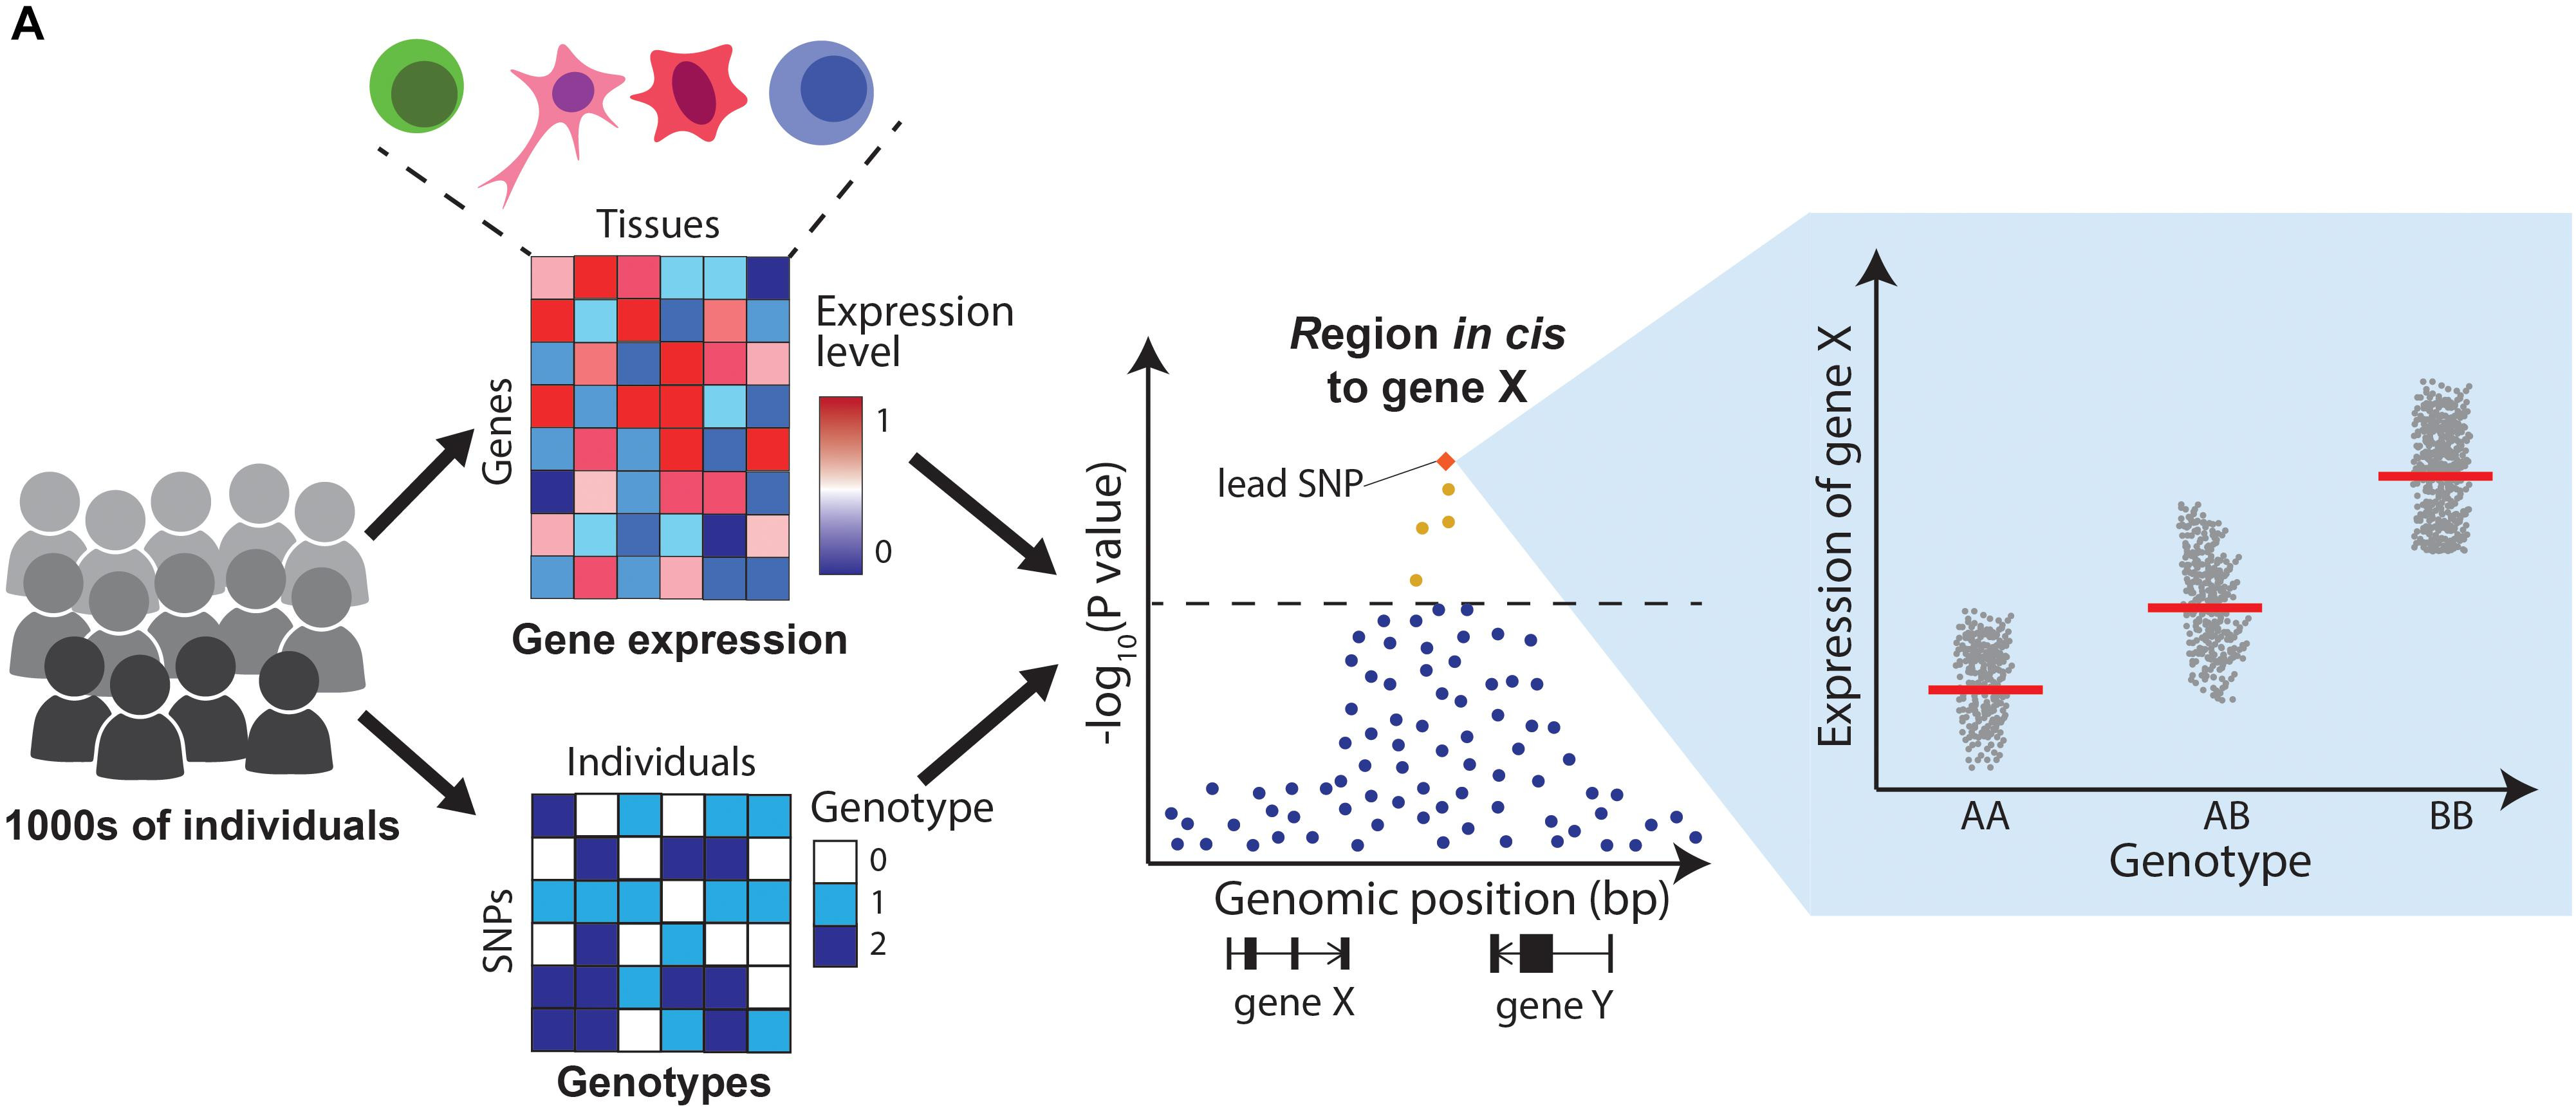
\includegraphics[width=\textwidth]{../presentation_230120_gold2022_paris/fig/doi_10.3389_fgene.2020.00424_fig4a.jpg}
        \end{center}
%
%        To my knowledge, it is unknown where are the most pleiotropice Eqtls in the genome.
%        This is important because this would give hints to putatitve pleiotropi genes (unknown or unknown) that are regulated by these pleiotropic eQTLs?
        Pleiotropy of eQTLs in genome is currently unknown

        \blfootnote{Cano-Gamez et al. 2020. doi:10.3389/fgene.2020.00424}
    \end{frame}

%%%%%%%%%%%%%%%%%%%%%%%%%%%%%%%%%%%%%%%%%%%%%%%%%%%%%%%%%%%%%%%%%%%%%%%%%%%%%%%%
    \begin{frame}
        \frametitle{Objectives}

        \begin{enumerate}
            \item To identify pleiotropic eQTLs in the genome
            \item To characterise the causes of their pleiotropy
        \end{enumerate}
    \end{frame}

%%%%%%%%%%%%%%%%%%%%%%%%%%%%%%%%%%%%%%%%%%%%%%%%%%%%%%%%%%%%%%%%%%%%%%%%%%%%%%%%
    \begin{frame}
        \frametitle{Strategy}

        \begin{enumerate}
            \item Annotate eQTLs with GWAS traits (Colocalization analysis)
            \item Define categories for GWAS traits
            \item Aggregate categories of eQTLs: Pleiotropic eQTLs
            \item Aggregate pleiotropic eQTLs in genome regions
            \item Explore properties pleiotropic eQTLs and regions
        \end{enumerate}
    \end{frame}

%%%%%%%%%%%%%%%%%%%%%%%%%%%%%%%%%%%%%%%%%%%%%%%%%%%%%%%%%%%%%%%%%%%%%%%%%%%%%%%%
    \begin{frame}
        \frametitle{Colocalization to annotate eQTLs with GWAS traits}

        \begin{columns}
            \begin{column}{0.5\textwidth}
                \begin{center}
                    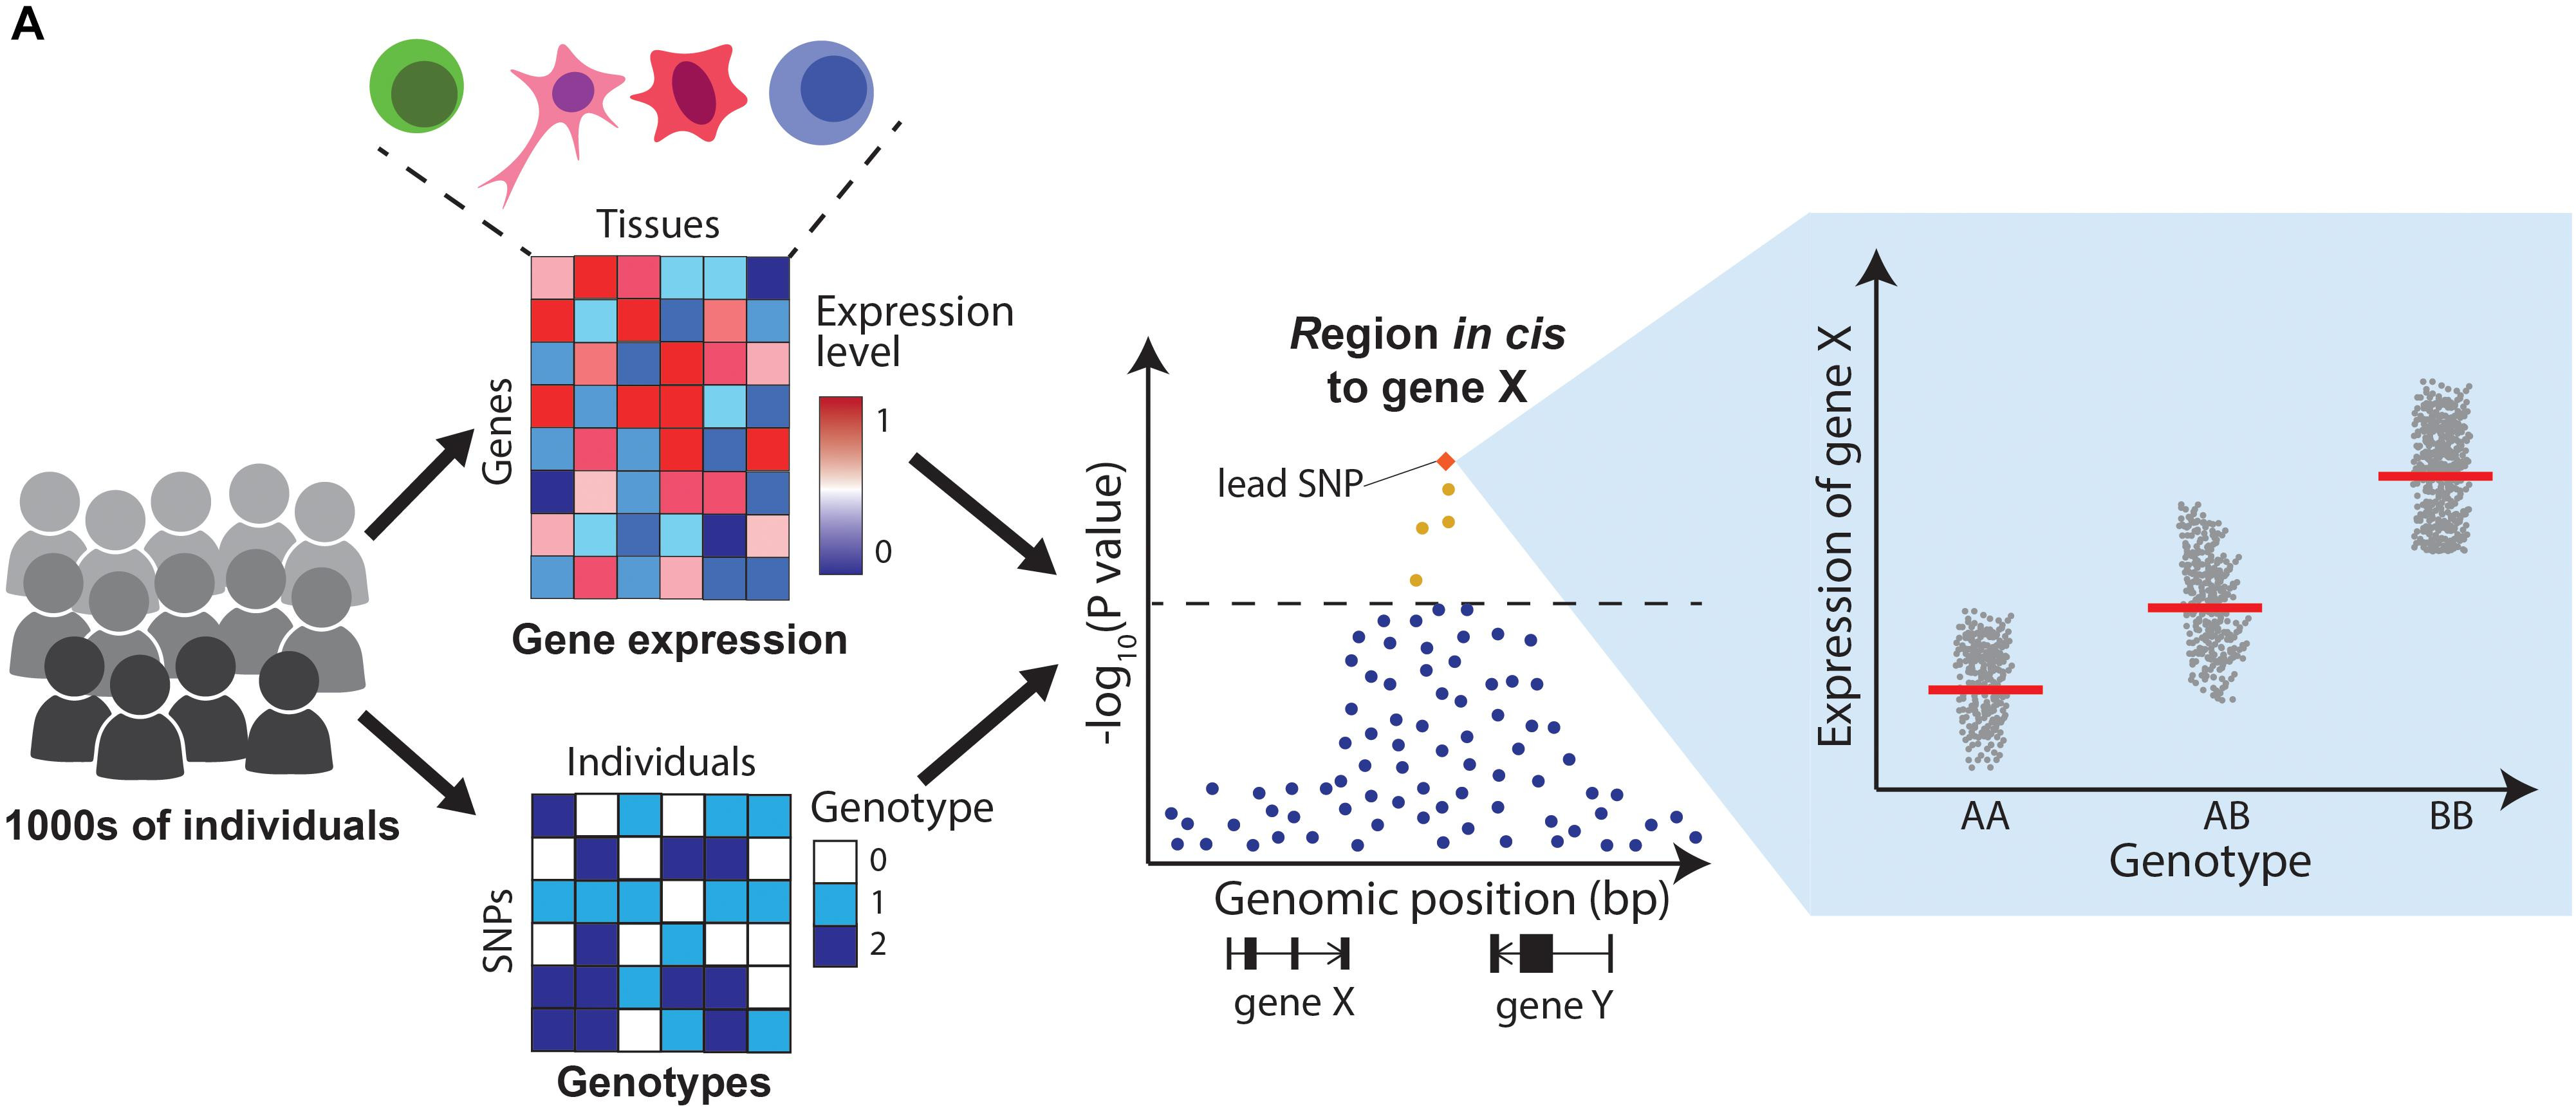
\includegraphics[width=\textwidth]{../presentation_230120_gold2022_paris/fig/doi_10.3389_fgene.2020.00424_fig4a.jpg}
                \end{center}
            \end{column}
            \begin{column}{0.5\textwidth}
                \begin{center}
                    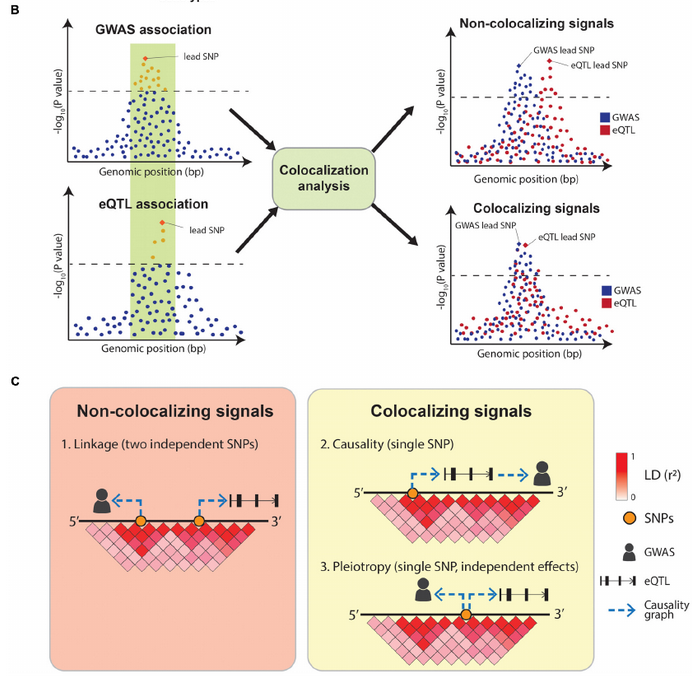
\includegraphics[width=\textwidth]{../presentation_230120_gold2022_paris/fig/doi_10.3389_fgene.2020.00424_fig4bc.png}
                \end{center}
            \end{column}
        \end{columns}

        \blfootnote{Cano-Gamez et al. 2020. doi:10.3389/fgene.2020.00424}
    \end{frame}

%%%%%%%%%%%%%%%%%%%%%%%%%%%%%%%%%%%%%%%%%%%%%%%%%%%%%%%%%%%%%%%%%%%%%%%%%%%%%%%%
    \begin{frame}
        \frametitle{IEA OpenGWAS database\footnote{https://gwas.mrcieu.ac.uk}}

        \begin{itemize}
            \item UK biobank, GWAS catalog, Other datasets
            \item Physiological and disease traits
            \item 418 GWAS, based on sample size and traits
        \end{itemize}

    \end{frame}

%%%%%%%%%%%%%%%%%%%%%%%%%%%%%%%%%%%%%%%%%%%%%%%%%%%%%%%%%%%%%%%%%%%%%%%%%%%%%%%%
    \begin{frame}
        \frametitle{EBI eQTLs database\footnote{https://www.ebi.ac.uk/eqtl}}

        \begin{itemize}
            \item GTEX, DICE, ...
            \item Tissues, cell types, stimulated conditions, ...
            \item 127 studies in human from different datasets
        \end{itemize}

    \end{frame}

%%%%%%%%%%%%%%%%%%%%%%%%%%%%%%%%%%%%%%%%%%%%%%%%%%%%%%%%%%%%%%%%%%%%%%%%%%%%%%%%
    \begin{frame}
        \frametitle{CRAN - Package coloc\footnote{https://cran.r-project.org/web/packages/coloc/index.html}}

        \begin{itemize}
            \item Colocalisation analysis of GWAS/eQTL with one causal variant
        \end{itemize}

        \begin{center}
            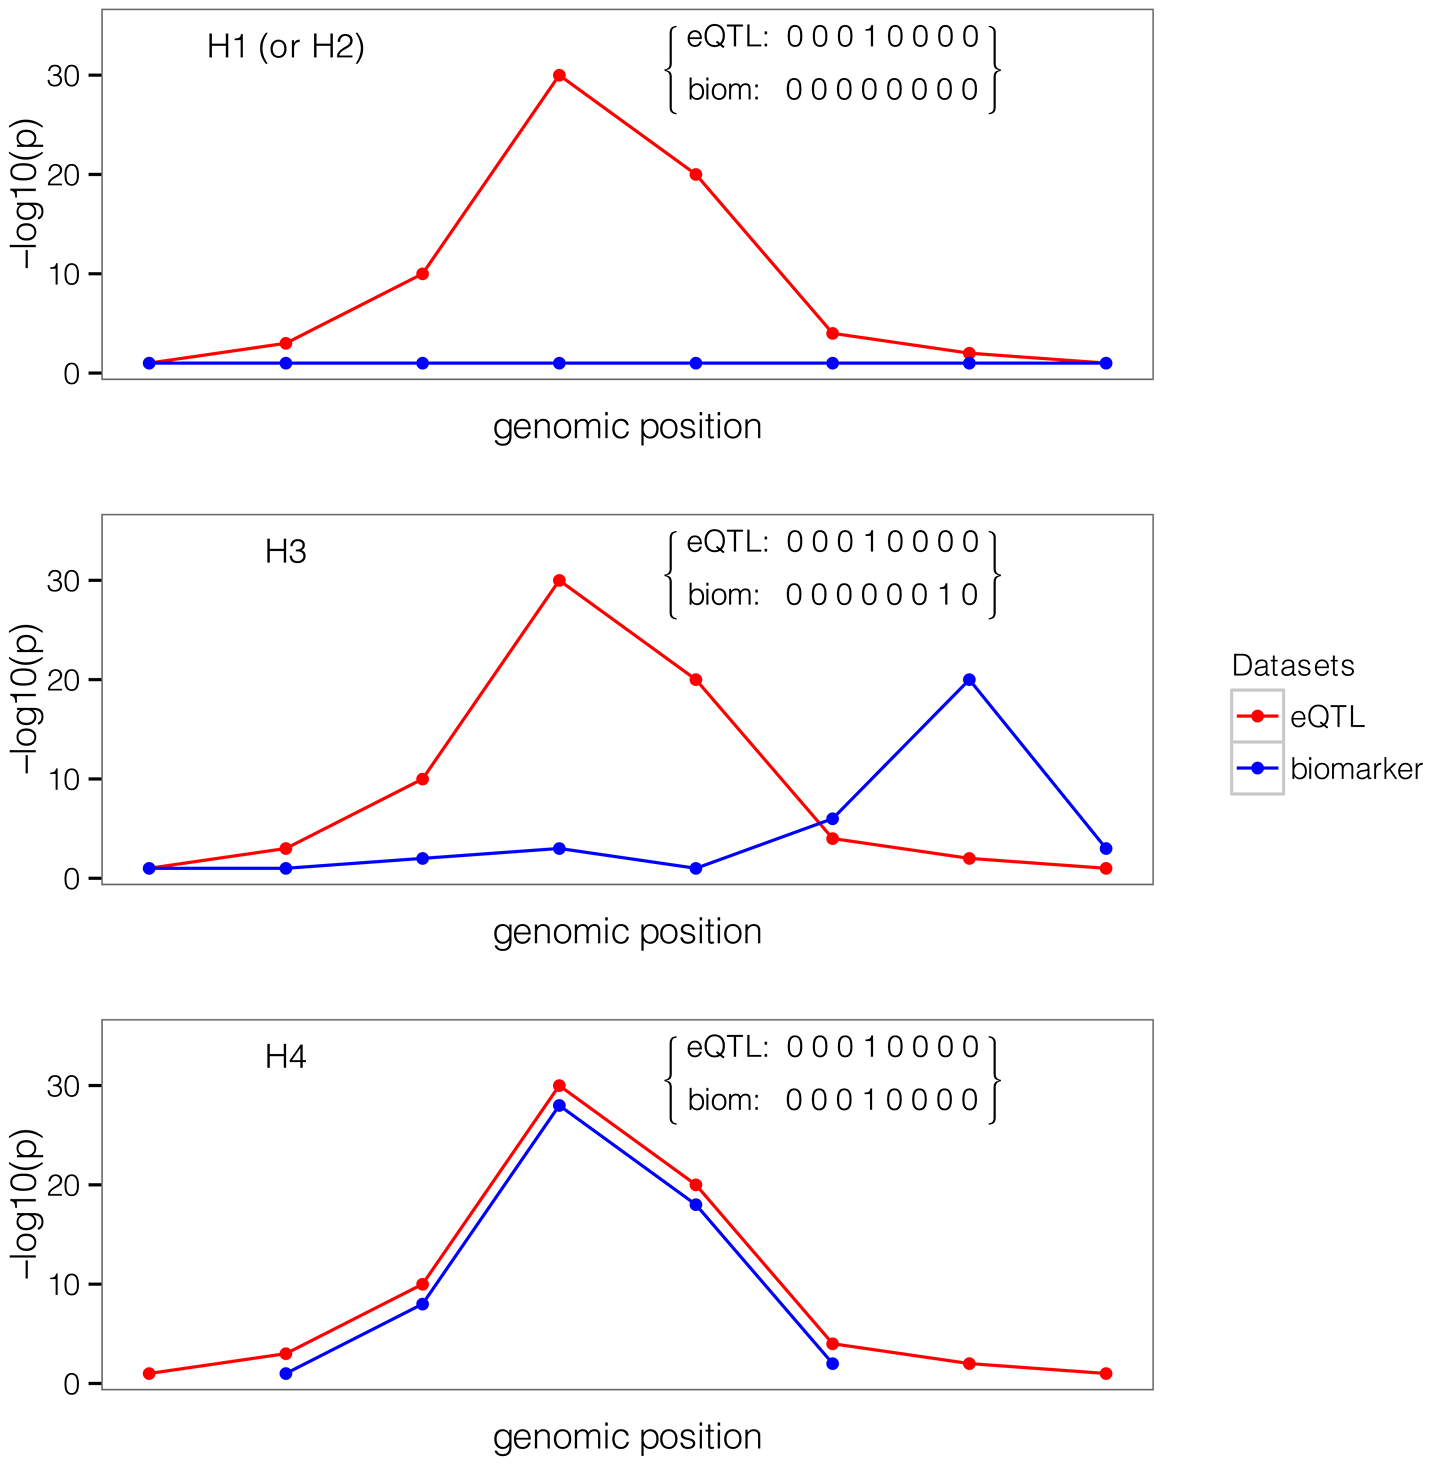
\includegraphics[width=0.5\textwidth]{../presentation_230120_gold2022_paris/fig/pgen.1004383.g001.png}
        \end{center}

    \end{frame}

    \section{Results}

%%%%%%%%%%%%%%%%%%%%%%%%%%%%%%%%%%%%%%%%%%%%%%%%%%%%%%%%%%%%%%%%%%%%%%%%%%%%%%%%
    \begin{frame}
        \frametitle{Colocalization of GWAS and eQTLs}

%In this project, I have carried a large colocalization analysis between ~300 GWAS traits and 127 eQTL studies belonging to different tissues and mainly primary cell types.
%In addition, by colocalizing statistically eQTLs and GWAS, we can to some extent, break, linkage disequilibrium

        \begin{itemize}
            \item Colocalization between 293 GWAS and 127 eQTL studies
        \end{itemize}

        \begin{figure}[!]
            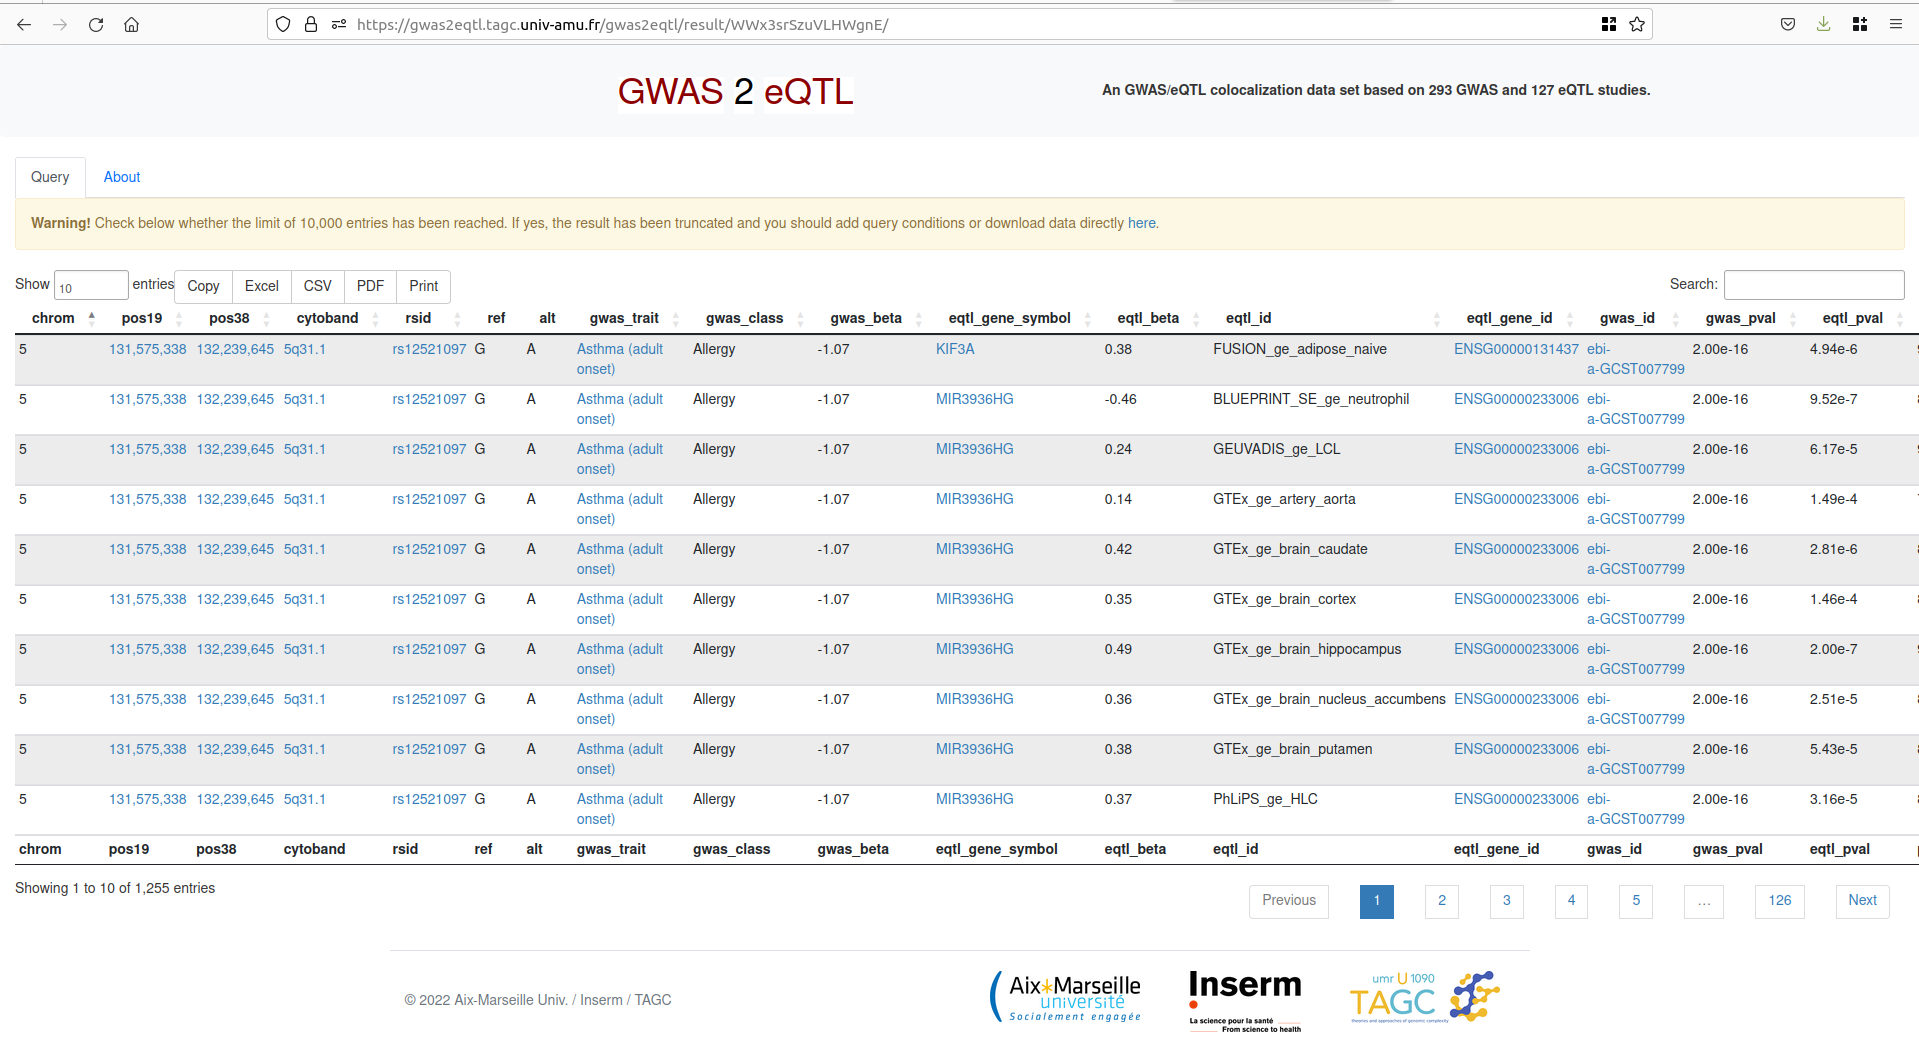
\includegraphics[width=\textwidth]{fig/web_portal.png}\label{fig:coloc_web}
        \end{figure}

    \end{frame}

%%%%%%%%%%%%%%%%%%%%%%%%%%%%%%%%%%%%%%%%%%%%%%%%%%%%%%%%%%%%%%%%%%%%%%%%%%%%%%%%
    \begin{frame}
        \frametitle{Large scale GWAS/eQTL colocalization analysis}

%In this project, I have carried a large colocalization analysis between ~300 GWAS traits and 127 eQTL studies belonging to different tissues and mainly primary cell types.
%In addition, by colocalizing statistically eQTLs and GWAS, we can to some extent, break, linkage disequilibrium

        \begin{itemize}
            \item Colocalization between 293 GWAS and 127 eQTL studies
            \item 25\%\footnote{SNP.PP.H4$\geq$0.5} of 10,000 leading SNPs, colocalized with at least one eQTL
            \item 5,000 eQTLs and 5,000 target genes\footnote{SNP.PP.H4$\geq$0.5}
            \item 138e3 colocalized variants with probability $\geq$ 0.75
            \item Percentage of GWAS loci explained by eQTL: histogram
        \end{itemize}

        \begin{figure}[!]
            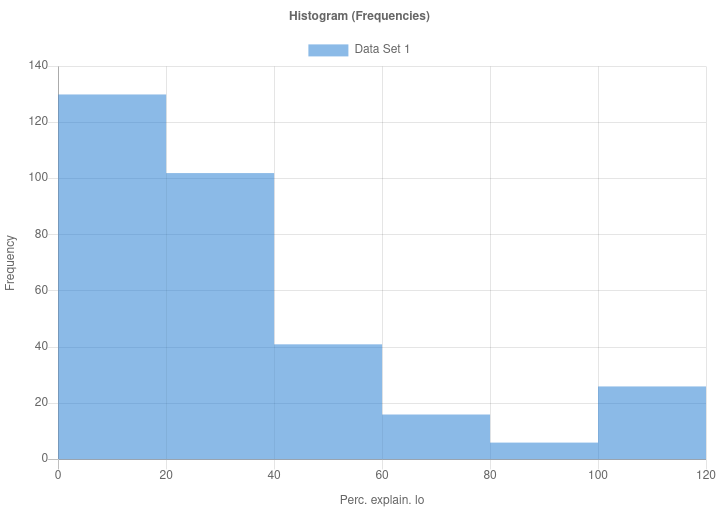
\includegraphics[width=0.5\textwidth]{fig/histogram_explained.png}\label{fig:perc_explained}
        \end{figure}

    \end{frame}

%%%%%%%%%%%%%%%%%%%%%%%%%%%%%%%%%%%%%%%%%%%%%%%%%%%%%%%%%%%%%%%%%%%%%%%%%%%%%%%%
    \begin{frame}
        \frametitle{Do GWAS traits cluster coherently?}

%        To evaluate the coherence of the colocalization data, I have computed distances between traits based on the Spearman correlation of the betas of the eqtl-gene-tissue

        GWAS distance based on correlation of beta of colocalized eQTL gene and tissue

        \begin{figure}[!]
            \includegraphics[width=0.5\textwidth]{\floatRelativePath/plthtmp_disease_comorbidity_matrix.py/corr_inkscape.png}
        \end{figure}

        \begin{itemize}
            \item Categories are coherent
            \item Help categorize GWAS traits
        \end{itemize}

%        In this heatmap, we can see that similar traits cluster together
%One difficulty for analysing pleiotropy is to distinguish similar traits for really different traits.
%In the previous heatmap, we have seen that traits cluster around coherent categories
%To look for real pleiotropic eQTLs I have manually annotated traits in different categories, such as cardiovascular disease, allergic, autoimmune, ....

    \end{frame}

%%%%%%%%%%%%%%%%%%%%%%%%%%%%%%%%%%%%%%%%%%%%%%%%%%%%%%%%%%%%%%%%%%%%%%%%%%%%%%%
%\begin{frame}
%\frametitle{Diseases?}
%
%\begin{table}[!tbp]
%\centering
%\scriptsize
%\hline
%\csvreader[separator=tab,
%tabular=ccrrp{0.4\textwidth},
%head,
%table head=\bfseries Chrom. & \bfseries Cytoband & \bfseries Pos (hg38) & \bfseries Variant & \bfseries GWAS Categories\\\hline,
%]{\floatRelativePath/cmpt_count_per_rsid.py/count_per_rsid_gwas_ms.tsv}{}% use head of csv as column names
%{\csvcoli\ & \csvcolii\ & \csvcoliii\ & \csvcoliv & \csvcolv}% specify your coloumns here
%\hline
%%
%\vspace{15pt}
%%
%\caption{Colocalized eQTL/GWAS variants involved in 5 or more GWAS categories. Genomic coordinates are given for the hg38 assembly. }\label{tab:pleitropic_variants}
%\end{table}
%
%\end{frame}

%%%%%%%%%%%%%%%%%%%%%%%%%%%%%%%%%%%%%%%%%%%%%%%%%%%%%%%%%%%%%%%%%%%%%%%%%%%%%%%%
    \begin{frame}
        \frametitle{How are pleiotropic eQTLs defined?}

        \begin{itemize}
            \item Annotate GWAS traits uniformly with ontologies
            \item Annotate normalized trait name in higher-level categories, eg cardiovascular
            \item Group categories of each eQTL
            \item Analyse eQTLs in groups based on the number of trait categories
        \end{itemize}

    \end{frame}

%%%%%%%%%%%%%%%%%%%%%%%%%%%%%%%%%%%%%%%%%%%%%%%%%%%%%%%%%%%%%%%%%%%%%%%%%%%%%%%%
    \begin{frame}
        \frametitle{Most pleiotroic eQTLs}

        \begin{itemize}
            \item Example pleiotropic eQTLs in different cytobands
            \item The representative gene is the eQTL gene with the highest PubMed publication count
        \end{itemize}

% full size table is table
        \begin{table}[!tbp]
            \centering
            \footnotesize
            \csvreader[separator=tab,
            tabular=crclcp{0.4\textwidth},
            head,
            table head=\bfseries Chrom. & \bfseries Pos (hg38) & \bfseries Cytoband & \bfseries RSID & \bfseries Known eQTL gene & \bfseries GWAS Categories\\\hline,
            ]{\floatRelativePath/cmpt_count_per_rsid.py/count_per_rsid_gwas_ms.tsv}{}% use head of csv as column names
                {\csvcoli\ & \csvcolii\ & \csvcoliii\ & \csvcoliv\ & \csvcolv\ & \csvcolvi}% specify your coloumns here
            \vspace{15pt}\label{tab:pleitropic_variants}
        \end{table}

    \end{frame}

%%%%%%%%%%%%%%%%%%%%%%%%%%%%%%%%%%%%%%%%%%%%%%%%%%%%%%%%%%%%%%%%%%%%%%%%%%%%%%%%
\begin{frame}
    \frametitle{How are pleiotropic variants distributed?}

    \begin{columns}
        \begin{column}{0.32\textwidth}
            \begin{center}
                \includegraphics[width=\textwidth]{\floatRelativePath/pltsctr_x_per_rsid_y_gwas.py/count_per_rsid_chr5_start132239645_end132497907_categories9.png}
            \end{center}
        \end{column}
        \begin{column}{0.32\textwidth}
            \begin{center}
                \includegraphics[width=\textwidth]{\floatRelativePath/pltsctr_x_per_rsid_y_egene.py/count_per_rsid_chr5_start132239645_end132497907_categories9.png}
            \end{center}
        \end{column}
        \begin{column}{0.32\textwidth}
            \begin{center}
                \includegraphics[width=\textwidth]{\floatRelativePath/pltsctr_x_per_rsid_y_etissue.py/count_per_rsid_chr5_start132239645_end132497907_categories9.png}
            \end{center}
        \end{column}
    \end{columns}

    \begin{center}
        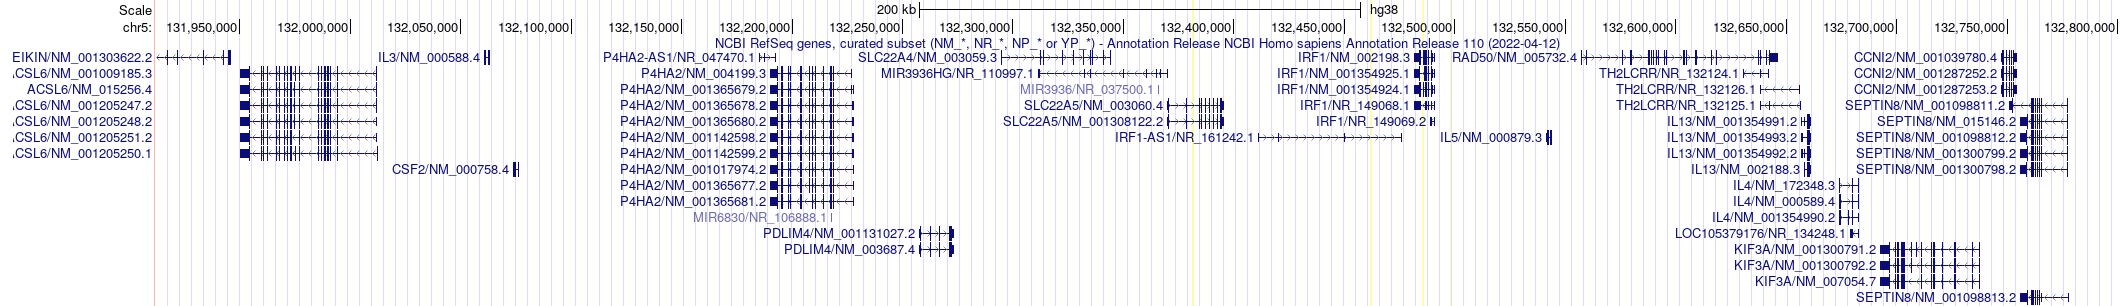
\includegraphics[width=\textwidth]{../presentation_230120_gold2022_paris/fig/chr5_131912097_132802472.png}
    \end{center}

    \small
    \begin{itemize}
        \item The cytokine locus: chr5:131,912,097-132,802,472. Genes IRF1, IL3, IL4, IL5, ...
        \item Diseases: Allergy,Autoimmune dis.,Cancer of breast,Circulatory sys. dis.,Hypertension,Respiratory system dis.
        \item For instance: rs2522051 regulates 12 e-genes in 23 e-tissues
    \end{itemize}
    \normalsize

\end{frame}

%%%%%%%%%%%%%%%%%%%%%%%%%%%%%%%%%%%%%%%%%%%%%%%%%%%%%%%%%%%%%%%%%%%%%%%%%%%%%%%%
    \begin{frame}
        \frametitle{Does trait categories correlate with eQTL and biosample counts?}

        \begin{figure}[!]
            \includegraphics[width=0.5\textwidth]{\floatRelativePath/cmpt_count_per_rsid.py/count_per_rsid_gwas_egene_etissue_corr}\label{fig:count_per_rsid_gwas_egene_etissue_corr}
        \end{figure}

    \end{frame}

%%%%%%%%%%%%%%%%%%%%%%%%%%%%%%%%%%%%%%%%%%%%%%%%%%%%%%%%%%%%%%%%%%%%%%%%%%%%%%%%
    \begin{frame}
        \frametitle{Most pleiotroic regions}

% full size table is table
        \begin{table}[!tbp]
            \centering
            \footnotesize
%\hline
            \csvreader[
                separator=tab,
                tabular=p{0.005\textwidth}p{0.05\textwidth}p{0.05\textwidth}p{0.05\textwidth}p{0.05\textwidth}p{0.5\textwidth},
                head,
                table head=\bfseries Chr. & \bfseries Start & \bfseries End & \bfseries Cytob. & \bfseries Known eQTL gene & \bfseries GWAS Categories\\\hline,
            ]{\floatRelativePath/cmpt_pleiotropic_regions.py/100000/region_window_ms.tsv}{}% use head of csv as column names
            {\csvcoli\ & \csvcolii\ & \csvcoliii\ & \csvcoliv\ & \csvcolv\ & \csvcolvi}% specify your coloumns here
%\hline
%
            \vspace{15pt}
            \caption{Pleiotropic regions involving 6 or more GWAS classes. These regions were built with a sliding window of 1e5 nt. Genomic coordinates are given for the hg38 assembly.}\label{tab:pleiotropic_regions}
        \end{table}

    \end{frame}

%%%%%%%%%%%%%%%%%%%%%%%%%%%%%%%%%%%%%%%%%%%%%%%%%%%%%%%%%%%%%%%%%%%%%%%%%%%%%%%%%
%    \begin{frame}
%        \frametitle{The IRF1/IL4 locus}
%
%        \begin{figure}[!]
%            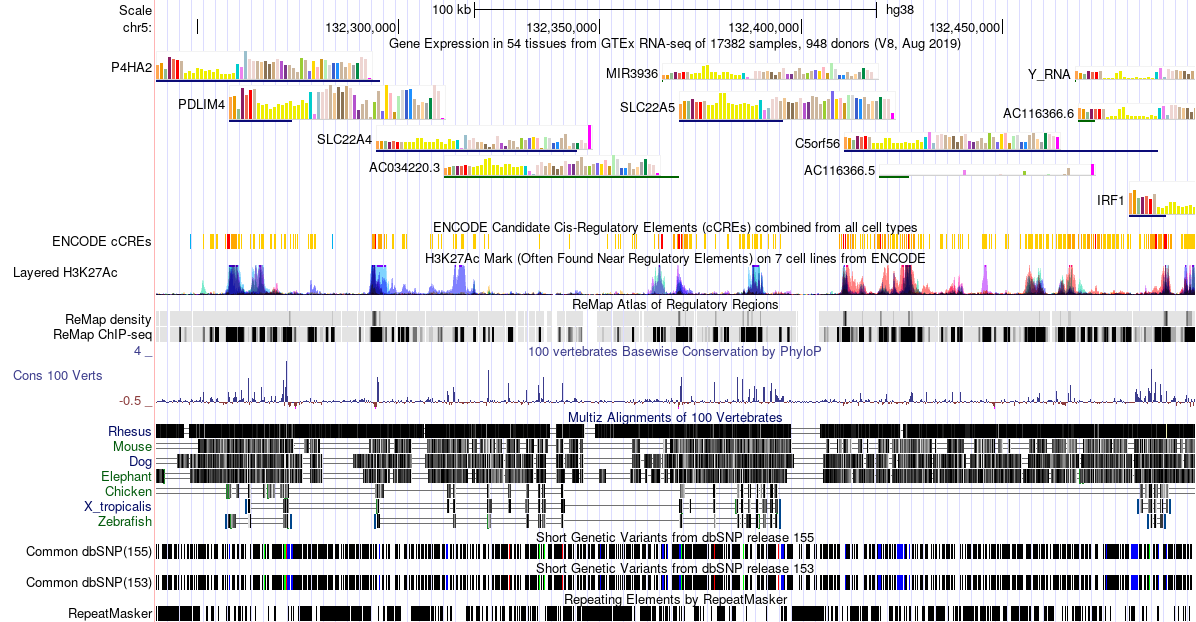
\includegraphics[width=0.95\textwidth]{fig/il4}
%        \end{figure}
%
%        \begin{itemize}
%            \item Sevaral immune genes
%            \item GWAS categories: allergic disease; autoimmune disease; body height; breast cancer; cancer; cardiovascular disease; hypertensive disorder; respiratory system disease; skin disease
%            \item eQTL biosamples: adipose tissue;aorta;blood;brain;breast; ...
%        \end{itemize}
%
%    \end{frame}

%%%%%%%%%%%%%%%%%%%%%%%%%%%%%%%%%%%%%%%%%%%%%%%%%%%%%%%%%%%%%%%%%%%%%%%%%%%%%%%%
    \begin{frame}
        \frametitle{The CDKN2A/P16 locus}

        \begin{figure}[!]
            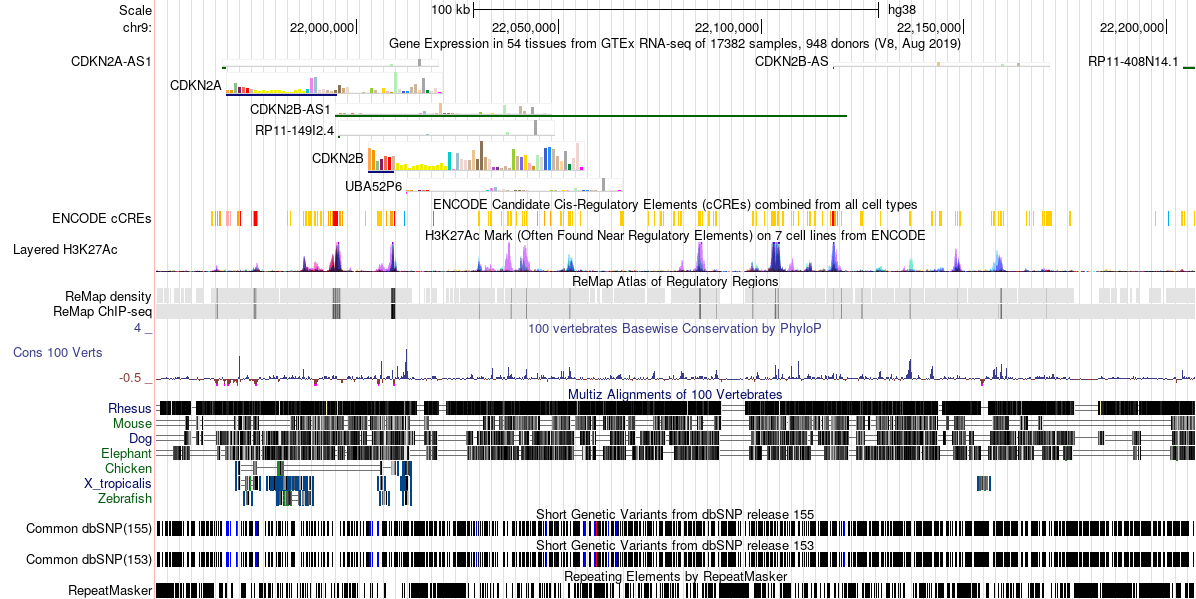
\includegraphics[width=0.95\textwidth]{fig/cdk2na}
        \end{figure}

        \begin{itemize}
            \item Cell cycle regulator
            \item Trait categories: cancer;cardiovascular disease;hypertensive disorder;joint disease;respiratory system disease;skin cancer
            \item eQTL biosamples: adipose tissue;blood;brain;colon;immune system; ...
        \end{itemize}

    \end{frame}

%%%%%%%%%%%%%%%%%%%%%%%%%%%%%%%%%%%%%%%%%%%%%%%%%%%%%%%%%%%%%%%%%%%%%%%%%%%%%%%%
    \begin{frame}
        \frametitle{The TP53 locus}

        \begin{figure}[!]
            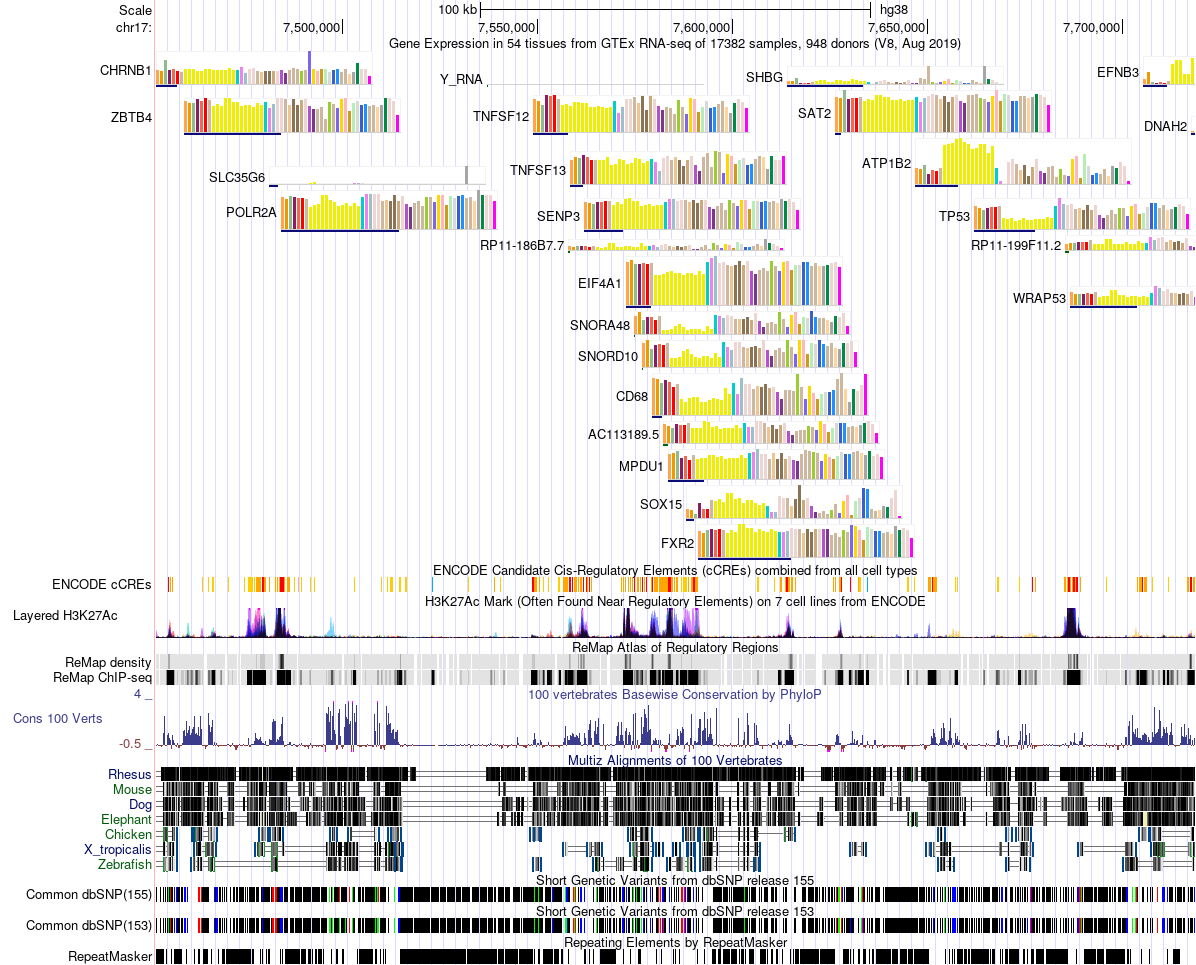
\includegraphics[width=0.95\textwidth]{fig/tp53}
        \end{figure}

        \begin{itemize}
            \item Cell cycle regulator
            \item Trait categories: cancer;cardiovascular disease;hypertensive disorder;joint disease;respiratory system disease;skin cancer
            \item eQTL biosamples: adipose tissue;adrenal gland;aorta;blood;brain; ...
        \end{itemize}

    \end{frame}

% %%%%%%%%%%%%%%%%%%%%%%%%%%%%%%%%%%%%%%%%%%%%%%%%%%%%%%%%%%%%%%%%%%%%%%%%%%%%%%%%
%     \begin{frame}
%         \frametitle{Where are the pleiotropic variants?\footnote{https://www.ensembl.org/vep}}
%
%         \begin{center}
%             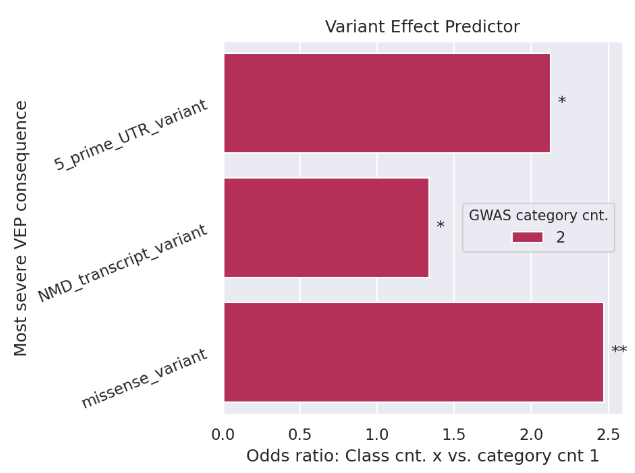
\includegraphics[width=0.7\textwidth]{fig/vep.png}
%         \end{center}
%
%         In the transcripts
%
% %        \let\thefootnote\relax\footnotetext{$^1$https://www.ensembl.org/vep}
%
%     \end{frame}

%%%%%%%%%%%%%%%%%%%%%%%%%%%%%%%%%%%%%%%%%%%%%%%%%%%%%%%%%%%%%%%%%%%%%%%%%%%%%%%%
    \begin{frame}
        \frametitle{Are pleiotropic eQTLs associated to more eQTL genes?}

        \begin{columns}
            \begin{column}{0.5\textwidth}
                \begin{center}
                    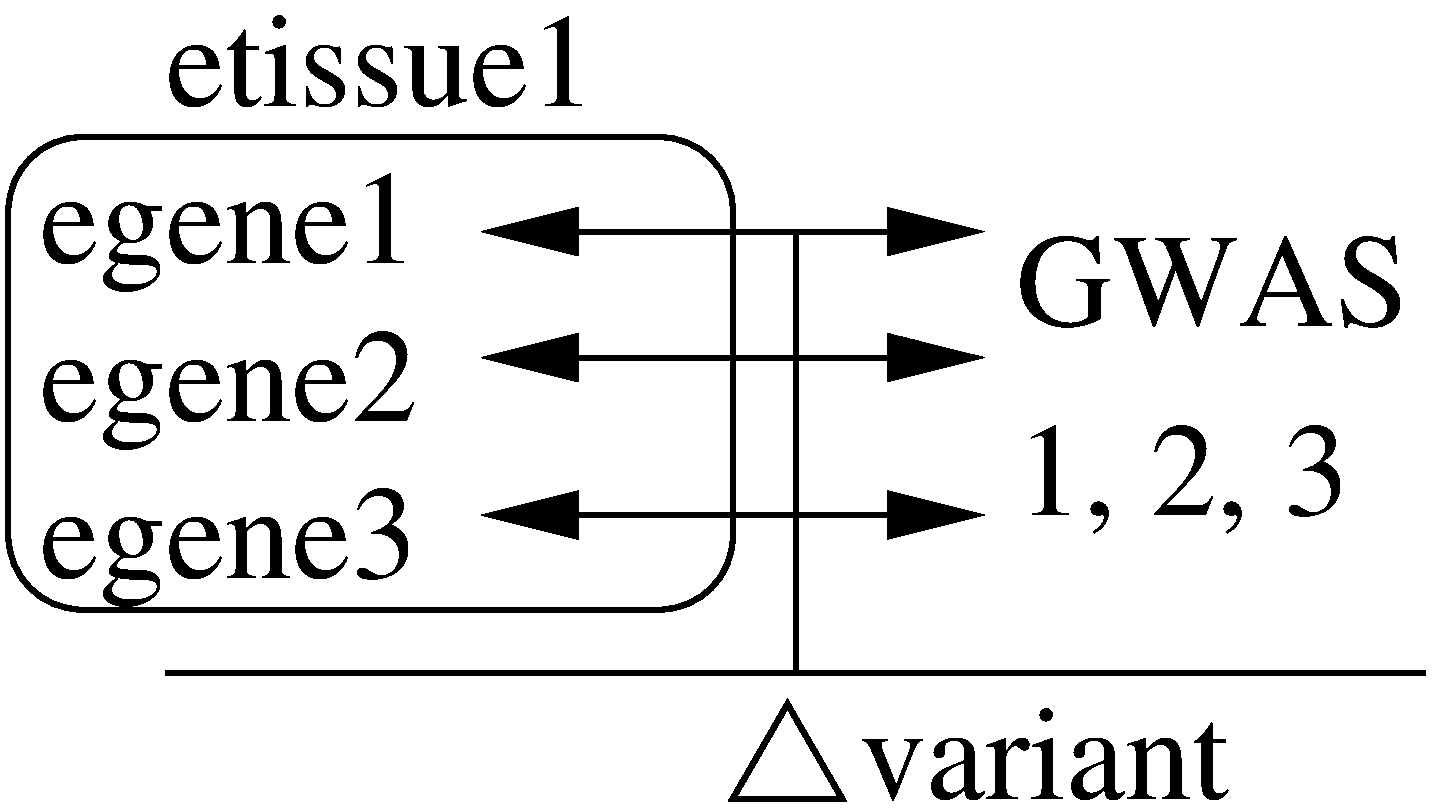
\includegraphics[width=0.7\textwidth]{../presentation_230120_gold2022_paris/fig/model_pleio_egenes.png}
                \end{center}
            \end{column}
            \begin{column}{0.5\textwidth}  %%<--- here
                \begin{center}
                    \includegraphics[width=\textwidth]{\floatRelativePath/pltbar_x_per_variant_etissue_y_egene.py/plt.png}
                \end{center}
            \end{column}
        \end{columns}

    \end{frame}

%%%%%%%%%%%%%%%%%%%%%%%%%%%%%%%%%%%%%%%%%%%%%%%%%%%%%%%%%%%%%%%%%%%%%%%%%%%%%%%%
    \begin{frame}
        \frametitle{Are pleiotropic eQTLs associated to more eQTL tissues?}

        \begin{columns}
            \begin{column}{0.5\textwidth}
                \begin{center}
                    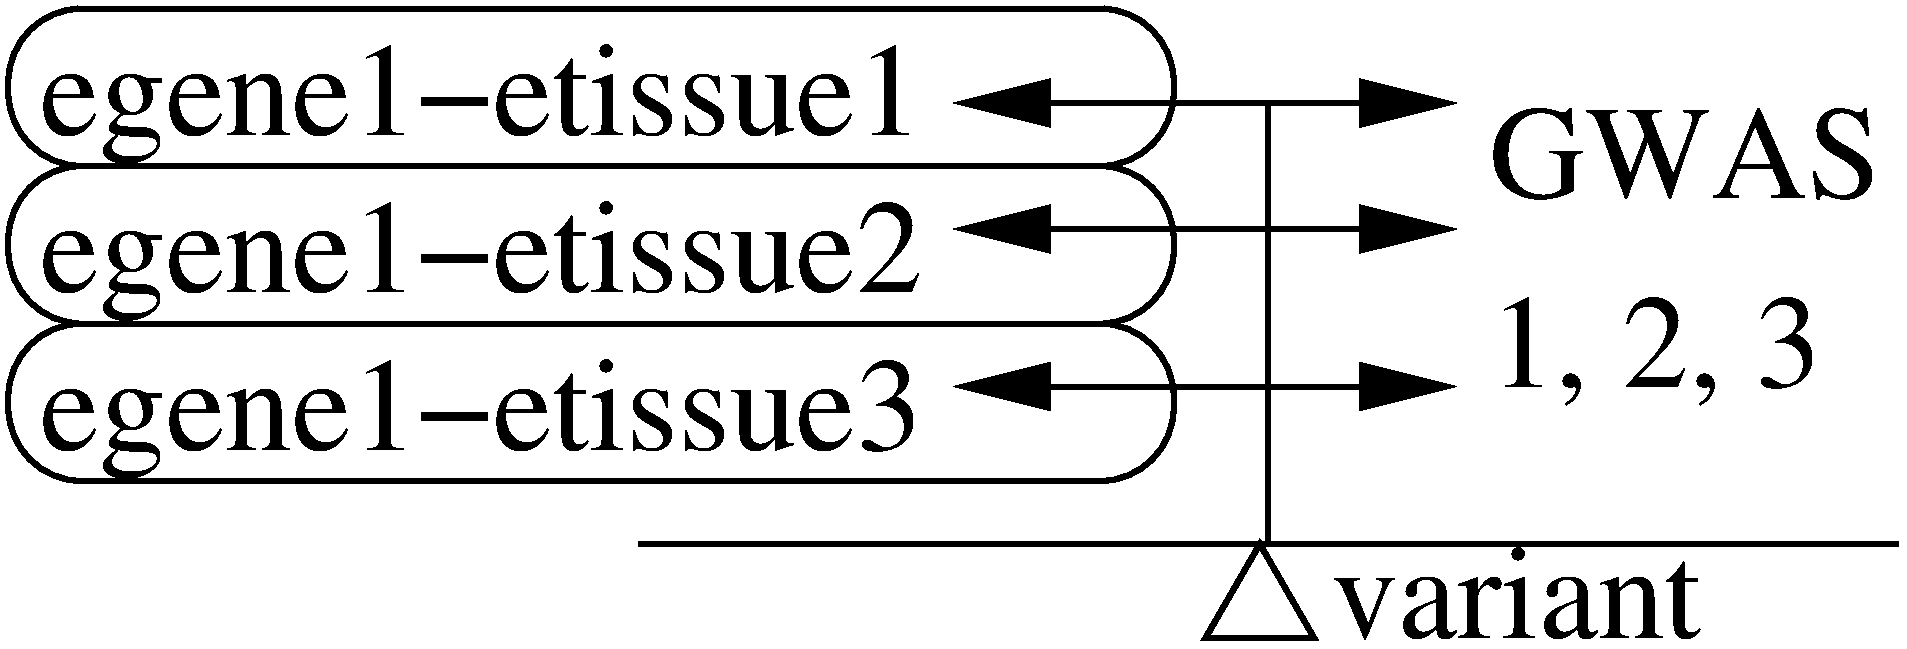
\includegraphics[width=0.7\textwidth]{../presentation_230120_gold2022_paris/fig/model_pleio_etissues.png}
                \end{center}
            \end{column}
            \begin{column}{0.5\textwidth}  %%<--- here
                \begin{center}
                    \includegraphics[width=\textwidth]{\floatRelativePath/pltbar_x_per_variant_egene_y_etissue.py/plt.png}
                \end{center}
            \end{column}
        \end{columns}

    \end{frame}

%%%%%%%%%%%%%%%%%%%%%%%%%%%%%%%%%%%%%%%%%%%%%%%%%%%%%%%%%%%%%%%%%%%%%%%%%%%%%%%%
    \begin{frame}
        \frametitle{Do pleiotropic eQTLs bind more transcription factors?\footnote{https://remap.univ-amu.fr}}

        \begin{columns}
            \begin{column}{0.5\textwidth}
                \begin{center}
                    \includegraphics[width=\textwidth]{\floatRelativePath/pltbox_x_per_rsid_y_remapnr.py/bxplt_remaptf_per_rsid_flank_10.png}
                \end{center}
            \end{column}
            \begin{column}{0.5\textwidth}  %%<--- here
                \begin{center}
                    \includegraphics[width=\textwidth]{\floatRelativePath/pltbar_x_per_variant_pleiotropy_y_remapcrm.py/remapcrm_flank10.png}
                \end{center}
            \end{column}
        \end{columns}

%        \let\thefootnote\relax\footnotetext{$^1$https://remap.univ-amu.fr}

    \end{frame}

%%%%%%%%%%%%%%%%%%%%%%%%%%%%%%%%%%%%%%%%%%%%%%%%%%%%%%%%%%%%%%%%%%%%%%%%%%%%%%%%
    \begin{frame}
        \frametitle{Web access}

        \url{https://gwas2eqtl.tagc.univ-amu.fr/gwas2eqtl/}

%These data can be useful to interpret disease variants
%        Therefore I have developed a small web portail

        \begin{figure}[!]
            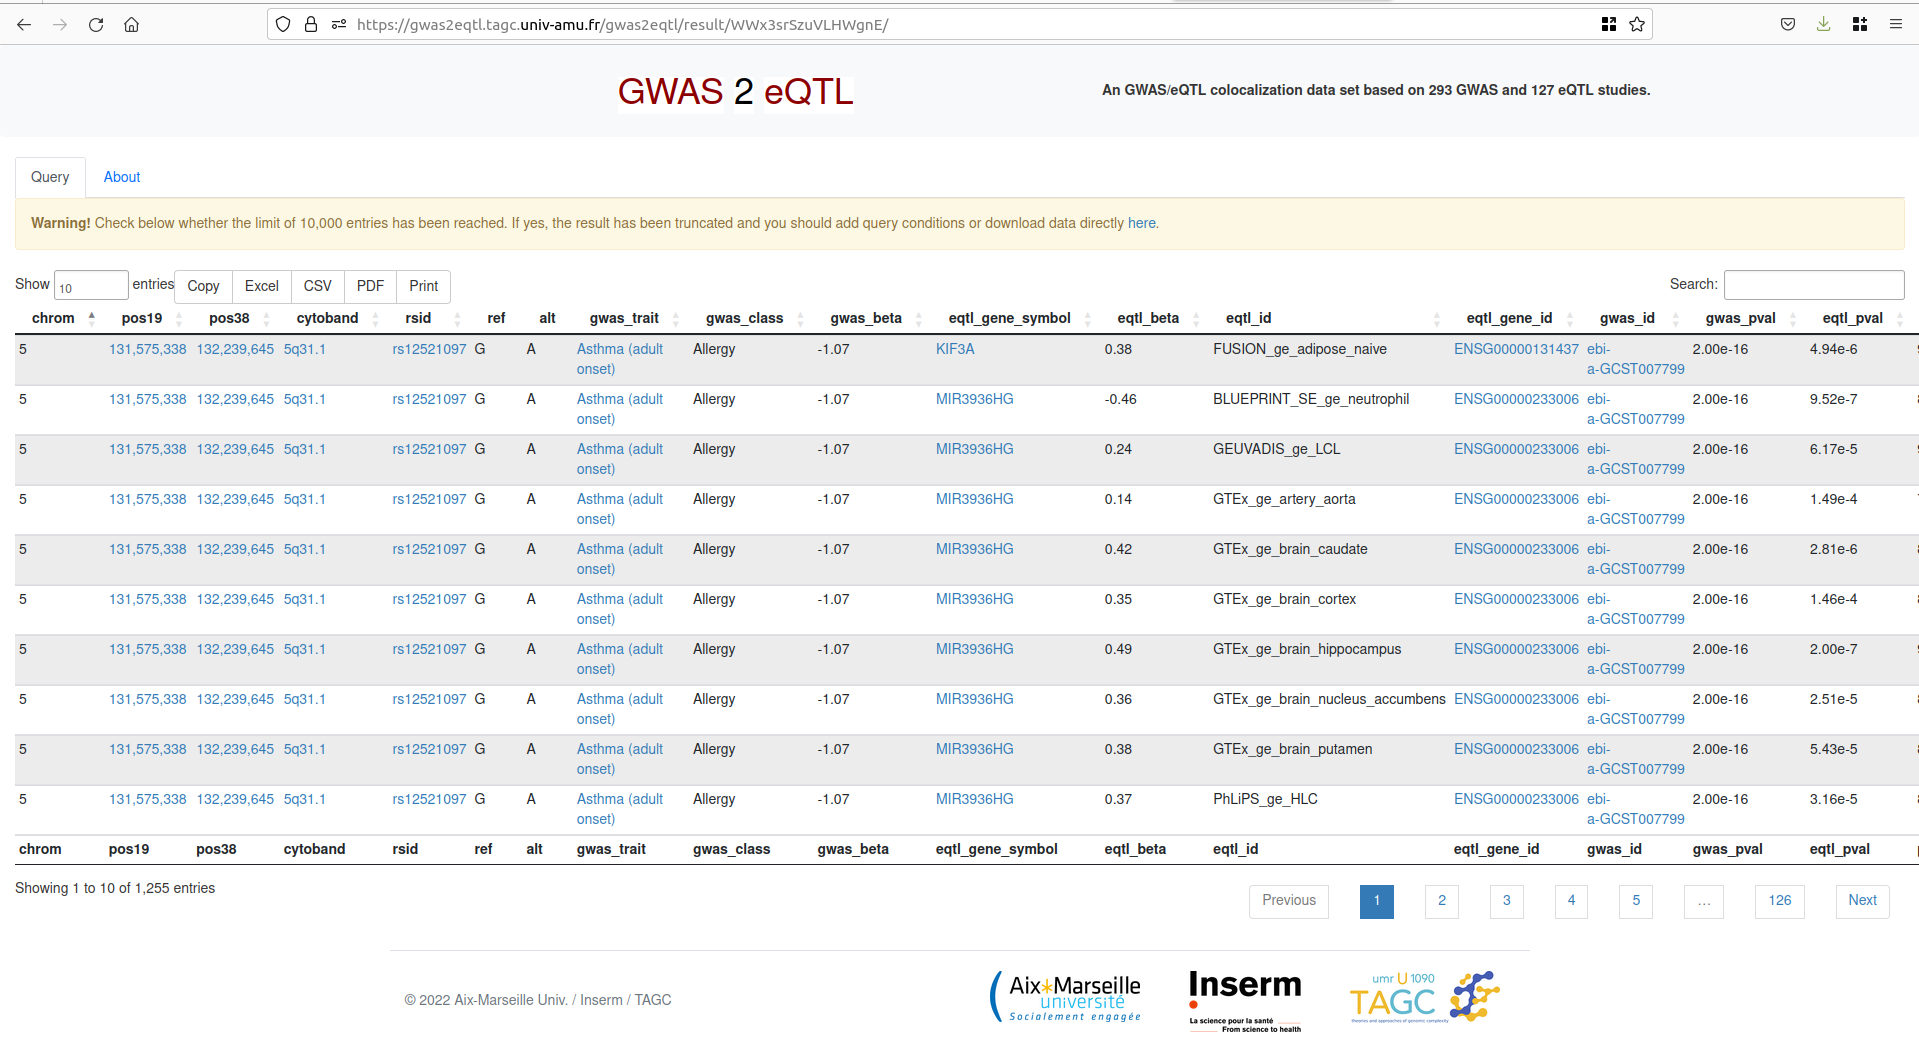
\includegraphics[width=\textwidth]{fig/web_portal.png}\label{fig:coloc_web}
        \end{figure}

    \end{frame}

    \section{Concluding remarks} %%%%%%%%%%%%%%%%%%%%%%%%%%%%%%%%%%%%%%%%%%%%%%%%%%%%%%%%%%%%%%

%%%%%%%%%%%%%%%%%%%%%%%%%%%%%%%%%%%%%%%%%%%%%%%%%%%%%%%%%%%%%%%%%%%%%%%%%%%%%%%%
    \begin{frame}
        \frametitle{Conclusion}

        \begin{itemize}
            \item A large set of GWAS variants annotated with putative target genes and tissues
            \item A list of pleiotropic eQTLs and regions
            \item Pleiotropic eQTL region include immune and cell cycle regulators
            \item Enrichment of 5' UTR and transcript (missense) variants
            \item Increased number of associated egenes and etissues
            \item A web site to access the data
        \end{itemize}

    \end{frame}

%%%%%%%%%%%%%%%%%%%%%%%%%%%%%%%%%%%%%%%%%%%%%%%%%%%%%%%%%%%%%%%%%%%%%%%%%%%%%%%%
    \begin{frame}
        \frametitle{Perspectives}

        \begin{itemize}
            \item Verify causality of eQTL genes on GWAS
            \item Analyze pleiotropic loci in more detail
        \end{itemize}

    \end{frame}

%%%%%%%%%%%%%%%%%%%%%%%%%%%%%%%%%%%%%%%%%%%%%%%%%%%%%%%%%%%%%%%%%%%%%%%%%%%%%%%%
    \begin{frame}
        \frametitle{Acknowledgements}

        \begin{itemize}
            \item L\'eopoldine Lecerf (M1)
            \item P Paul, P Rihet, M Michel, S Marquet, S Spicuglia
        \end{itemize}
%
        \vfill
%
        Funding
%
        \begin{itemize}
            \item Institut Cancer et Immunologie - Aix-Marseille Univ.
            \item Agence nationale de la recherche (ANR)
            \item GOLD
        \end{itemize}

    \end{frame}

%%%%%%%%%%%%%%%%%%%%%%%%%%%%%%%%%%%%%%%%%%%%%%%%%%%%%%%%%%%%%%%%%%%%%%%%%%%%%%%%
    \begin{frame}
        \frametitle{}

    \end{frame}

%%%%%%%%%%%%%%%%%%%%%%%%%%%%%%%%%%%%%%%%%%%%%%%%%%%%%%%%%%%%%%%%%%%%%%%%%%%%%%%%
%\begin{frame}
%    \frametitle{Do pleiotropic variants associate to more traits (after fixing egene-etissue)?}
%
%    \begin{columns}
%        \begin{column}{0.5\textwidth}
%            \begin{center}
%                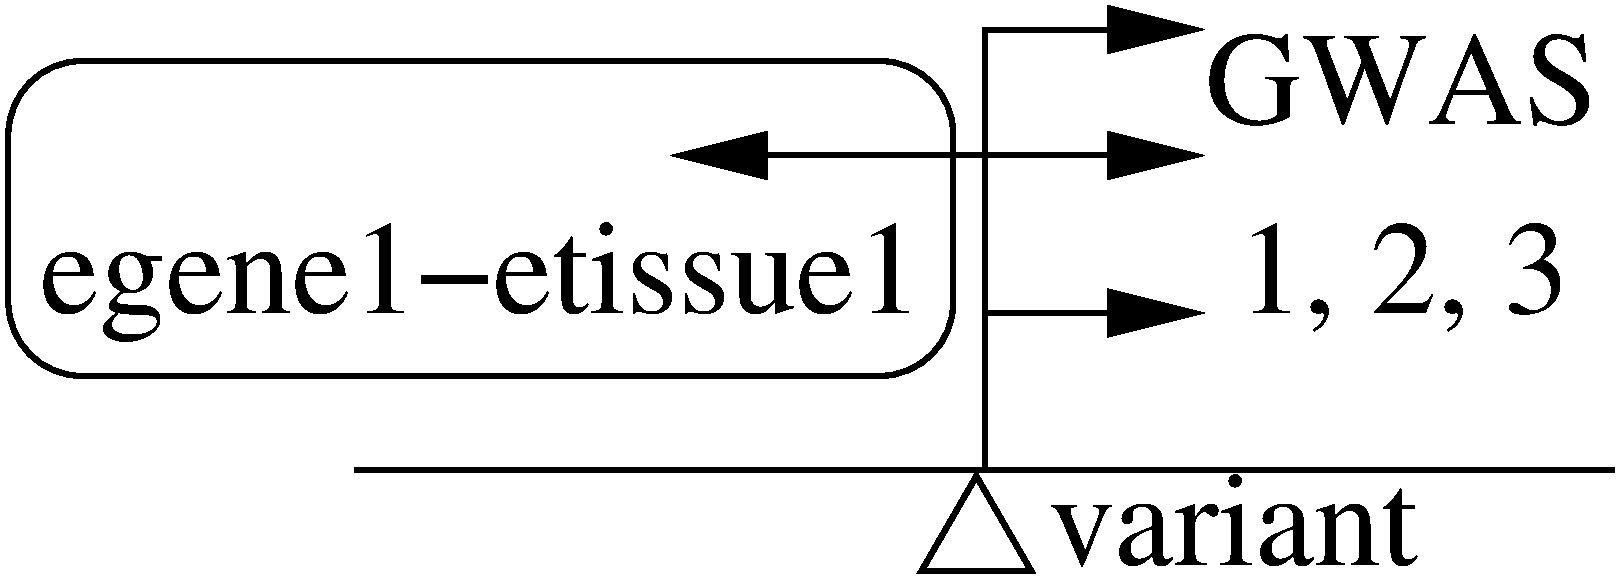
\includegraphics[width=0.7\textwidth]{../presentation_230120_gold2022_paris/fig/model_pleio_gwas.png}
%            \end{center}
%        \end{column}
%        \begin{column}{0.5\textwidth}  %%<--- here
%            \begin{center}
%                \includegraphics[width=\textwidth]{\floatRelativePath/pltbar_x_per_variant_egene_etissue_y_gwas.py/plt.png}
%            \end{center}
%        \end{column}
%    \end{columns}
%
%\end{frame}

\end{document}


